%% This is file `elsarticle-template-1-num.tex',
%%
%% Copyright 2009 Elsevier Ltd
%%
%% This file is part of the 'Elsarticle Bundle'.
%% ---------------------------------------------
%%
%% It may be distributed under the conditions of the LaTeX Project Public
%% License, either version 1.2 of this license or (at your option) any
%% later version.  The latest version of this license is in
%%    http://www.latex-project.org/lppl.txt
%% and version 1.2 or later is part of all distributions of LaTeX
%% version 1999/12/01 or later.
%%
%% Template article for Elsevier's document class `elsarticle'
%% with numbered style bibliographic references
%%
%% $Id: elsarticle-template-1-num.tex 149 2009-10-08 05:01:15Z rishi $
%% $URL: http://lenova.river-valley.com/svn/elsbst/trunk/elsarticle-template-1-num.tex $
%%
\documentclass[preprint,12pt]{elsarticle}

%% Use the option review to obtain double line spacing
%% \documentclass[preprint,review,12pt]{elsarticle}

%% Use the options 1p,twocolumn; 3p; 3p,twocolumn; 5p; or 5p,twocolumn
%% for a journal layout:
%% \documentclass[final,1p,times]{elsarticle}
%% \documentclass[final,1p,times,twocolumn]{elsarticle}
%% \documentclass[final,3p,times]{elsarticle}
%% \documentclass[final,3p,times,twocolumn]{elsarticle}
%% \documentclass[final,5p,times]{elsarticle}
%% \documentclass[final,5p,times,twocolumn]{elsarticle}

%% The graphicx package provides the includegraphics command.
\usepackage{graphicx}
%% The amssymb package provides various useful mathematical symbols
\usepackage{amssymb}
%% The amsthm package provides extended theorem environments
%% \usepackage{amsthm}
\usepackage{hyperref}

%% The lineno packages adds line numbers. Start line numbering with
%% \begin{linenumbers}, end it with \end{linenumbers}. Or switch it on
%% for the whole article with \linenumbers after \end{frontmatter}.
\usepackage{lineno}

%% natbib.sty is loaded by default. However, natbib options can be
%% provided with \biboptions{...} command. Following options are
%% valid:

%%   round  -  round parentheses are used (default)
%%   square -  square brackets are used   [option]
%%   curly  -  curly braces are used      {option}
%%   angle  -  angle brackets are used    <option>
%%   semicolon  -  multiple citations separated by semi-colon
%%   colon  - same as semicolon, an earlier confusion
%%   comma  -  separated by comma
%%   numbers-  selects numerical citations
%%   super  -  numerical citations as superscripts
%%   sort   -  sorts multiple citations according to order in ref. list
%%   sort&compress   -  like sort, but also compresses numerical citations
%%   compress - compresses without sorting
%%
%% \biboptions{comma,round}

% \biboptions{}

\journal{Journal Name}

\begin{document}

\begin{frontmatter}

%% Title, authors and addresses

\title{Go Fish and Probabilities}

%% use the tnoteref command within \title for footnotes;
%% use the tnotetext command for the associated footnote;
%% use the fnref command within \author or \address for footnotes;
%% use the fntext command for the associated footnote;
%% use the corref command within \author for corresponding author footnotes;
%% use the cortext command for the associated footnote;
%% use the ead command for the email address,
%% and the form \ead[url] for the home page:
%%
%% \title{Title\tnoteref{label1}}
%% \tnotetext[label1]{}
%% \author{Name\corref{cor1}\fnref{label2}}
%% \ead{email address}
%% \ead[url]{home page}
%% \fntext[label2]{}
%% \cortext[cor1]{}
%% \address{Address\fnref{label3}}
%% \fntext[label3]{}


%% use optional labels to link authors explicitly to addresses:
%% \author[label1,label2]{<author name>}
%% \address[label1]{<address>}
%% \address[label2]{<address>}

\author{Scott Munro}
\author{Andrew Gordineer}

\address{Austin, TX, United States}

\begin{abstract}
%% Text of abstract
Many people enjoy playing the card game Go Fish. Generally, the game is played by randomly guessing what cards a player’s opponents may or may not have. We set out to develop a system that uses probability to help player’s make better educated guesses. Using these educated guesses, we propose that a player's average win rate can be increased. 
\end{abstract}

\end{frontmatter}

%%
%% Start line numbering here if you want
%%
\linenumbers

%% main text
\section{Important Resources and Sources}
\label{P:1}
\noindent Project Source Code: 

\noindent \url{http://github.com/gordineerandrew/Go-Fish}

\noindent Mean and Std Deviation Tools: 

\noindent \url{https://www.easycalculation.com/statistics/standard-deviation.php}


\noindent Normal Curve Generator: 

\noindent\url{http://davidmlane.com/hyperstat/z_table.html}

\section{Logistics}
\label{P:2}

This project was developed using the Java programming lanuage and packages defined with the standard Java 7 SDK. Java was used for it's ability to rapidly prototype the GoFish simulation and to quickly develop simple object oriented designs. While other languages such as C can make more efficient use of the processor (which improves performance) and other languages such as Python or R are used in scientific fields, Java was chosen because the simulation is fairly lightweight and the ability to write code quickly outweighed the advantages of other languages. 

\section{GoFish Rules}
\label{P:3}
Because Go Fish is not explicitly defined anywhere, a set of guidelines and rules for our particular simulation of Go Fish must be established. 

\begin{itemize}
\item At the start of the game, each player is dealt seven cards, creating books as needed.
\item The game cycles in turns between each player until either a player loses all cards from their hand, or the deck is empty.
\item Each turn consists of a player requesting a card in their hand from an opposing player. If that player has the card, then the asking player is given that card to form a book, and that player gains a point. If the requested player does not have the card, then the asking player must “Go Fish!” and draw a card, ending their turn.
\item Books are comprised of a pair of cards with identical values (i.e. pair of two’s, ace’s etc). 
\item When the game is over a winner is determined by finding the player with either the maximum amount of books or, in the event of a tie, finding the player with no cards left in their hand.
\end{itemize}

\section{What We Accomplished}
\label{S:1}

We created a program that simulates the game of Go Fish, displaying the probabilities of each value of card for each of the players opponents. These probabilities are constantly updated based on events occurring in the game (i.e. Asking for cards, being asked for a card, handing over a card, making a book, and denying having a value). The AIPlayers play the game by randomly asking one of their opponents for a card that is currently in their hand. This version of AI is random, but representative of how people generally play GoFish, disregarding information that is gained through the game’s progression. A headless, logging mode was also established so that multiple iterations of the simulation could be run and recorded without needing explicit human input.

\subsection{Basic Control Flow Diagram}
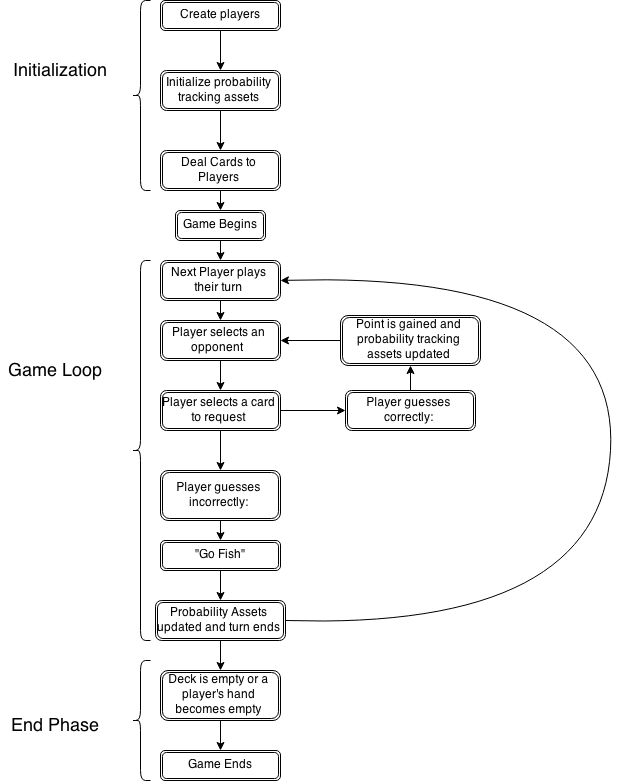
\includegraphics[scale=0.6]{../images/GoFishControlFlow.png}

\subsection{How Probability is Tracked}

The probability for each value of card is tracked by keeping a running count of the number of cards in each of the players opponent's hands known to not be that value. This is accomplished by incrementing the count each time a player gains a card (i.e. draws a card), decrementing the count whenever a player loses a card (i.e. makes a book or gives up a card to an opponent), and zeroing a card’s value if the player definitely doesn’t have that value (i.e. they have just formed a book or denied a request for the value). 

\subsection{How the Probability is Calculated}

The probability is calculated by using a combination of what is known about the unknown cards in a player’s hand that could be a specified value, the total number of unknown cards in the game that could be the specified value, and the number of cards of that value remaining in the game.
\vspace{5 mm}

\noindent Formula ($R$ = player being asked, $C$ = card being asked for)

\noindent$X$ = the number of cards in the R's hand that could be C

\noindent$Y$ = total unknown cards in the game that could be C

\noindent$Z$ = Number of C remaining in the game and not in your hand


\begin{equation}
\label{Probability}
\mbox{Pr(C in R’s Hand)} = \frac{X}Y * Z
\end{equation}


\subsection{Computer Simulated Players}

To appropriately simulate GoFish, multiple players are needed. To simplify the development of the simulation environment, the extra players are implemented as AI-Players instead of as other Human Players. Whereas the human player has to manually select a player and a card to ask for, the AI-Players randomly choose one of their opponents and a random card that exists in their hand during each of their turns. Aside from just acting as an extra player, these AI-Players act as a contrast to how the Human Player selects their cards. The Human Player can make educated guesses, but the AI-Player makes naive, random guesses that don’t adapt to the new information that is made available to every player as the game progresses. 

\subsection{Extension} 
This project could be extended in a few interesting ways. A better user interface could be developed that makes use of Graphical components. A variety of difficulties of AI could be created, taking advantage of the probability calculations being available and evolving their behavior based on the current state of the game.

\section{Experiment}
\label{S:2}
\subsection{Overview}
It can be accepted with common sense that having access to more information would positively affect a player's win rate, but it is an interesting challenge to see exactly how much it can benefit a player.

\subsection{Procedure}
To compare and contrast the naive strategy to our strategy with educated guesses, both needed to be tested in a standard way. The standard test we designed was to run the GoFish simulation with 4 players 10000 times and get the percentage of wins. This was repeated 1000 times and the results of these trials were used to generate a reliable mean and standard deviation. In turn these measures of central tendency can be used to form a normal curve to evaluate each strategy in comparison to each other.

\subsection{Data}
\begin{center}
	\begin{tabular}{l | l}
		Naive Strategy & Educated Strategy \\ \hline
		\textbf{$\mu$} = 28.604 & \textbf{$\mu$} = 67.0099  \\
		\textbf{$\sigma$} = 0.45955 & \textbf{$\sigma$} = 0.4698 \\ 
	\end{tabular}

	\vspace{4 mm}

	\textbf{$\mu$} = Mean

	\textbf{$\sigma$} = Standard Deviation

	\vspace{4 mm}

	\begin{tabular}{c c}
		
\includegraphics[scale=0.37]{../images/dumbCurve.png} & 
\includegraphics[scale=0.37]{../images/smartCurve.png} \\
	\end{tabular}

\end{center}

\subsection{Results}

The results are clear. Using the educated strategy with probability awarness results in winning twice as many rounds of Go Fish as using the naive strategy. Furthermore, the standard deviation of both strategies is so miniscule that there is virtually no chance that the naive strategy will ever deviate anywhere near the results of the educated strategy. The experiment has been proven successful.

\section{Some Challenges During Development}
\label{S:3}

\subsection{Learning about Go Fish}
Go Fish is not explicitly defined and is riddled with house rules, variations, and inconsistencies. To develop a proper simulation, a specific subset of rules had to be established and this set of rules needed to cohesively work with our project.

\subsection{Tracking the probability}
Giving different portions of our code the correct access to the correct information proved troublesome when we began trying to work from a strictly object oriented programming paradigm. A simpler, more imperative form of object oriented programming was adopted to fit our project. 

\subsection{Calculating Probability}
Determining a method of calculating the probabilities of each of the card values, without having to compute very intense functions proved to be difficult. Issues concerning whether or not the probabilities were to be distributed among opponents and how to consider a multitude of unknown cards made the problem difficult to conceptualize. 

\subsection{Designing the user interface}
Displaying the appropriate information to the user in an organized and readable manner proved difficult within a text-based interface. A lot of time was spent defining formatting standards and input delays so that a player could appropriately digest all of the information that would need to be presented to them.


%% The Appendices part is started with the command \appendix;
%% appendix sections are then done as normal sections
%% \appendix

%% \section{}
%% \label{}

%% References
%%
%% Following citation commands can be used in the body text:
%% Usage of \cite is as follows:
%%   \cite{key}          ==>>  [#]
%%   \cite[chap. 2]{key} ==>>  [#, chap. 2]
%%   \citet{key}         ==>>  Author [#]

%% References with bibTeX database:

\bibliographystyle{model1-num-names}
\bibliography{sample.bib}

%% Authors are advised to submit their bibtex database files. They are
%% requested to list a bibtex style file in the manuscript if they do
%% not want to use model1-num-names.bst.

%% References without bibTeX database:

% \begin{thebibliography}{00}

%% \bibitem must have the following form:
%%   \bibitem{key}...
%%

% \bibitem{}

% \end{thebibliography}


\end{document}

%%
%% End of file `elsarticle-template-1-num.tex'.